\documentclass[conference]{IEEEtran}
\IEEEoverridecommandlockouts
\usepackage[hyphens]{url}
\usepackage{cite}
\usepackage{amsmath,amssymb,amsfonts}
\usepackage{algorithmic}
\usepackage{graphicx}
\usepackage{textcomp}
\usepackage{xcolor}
\usepackage{booktabs}
\usepackage{svg}
\usepackage{multirow}
\usepackage{listings}
\usepackage{fancybox}
\usepackage{tcolorbox}
\usepackage{tikz}
\usetikzlibrary{shapes.geometric, arrows.meta, positioning, calc, backgrounds, fit, shadows}

% Define colors for TikZ diagram
\definecolor{primary}{RGB}{70, 130, 180}   % SteelBlue
\definecolor{secondary}{RGB}{255, 140, 0}  % DarkOrange
\definecolor{tertiary}{RGB}{34, 139, 34}   % ForestGreen
\definecolor{neutral}{RGB}{240, 240, 240}  % LightGray
\definecolor{accent}{RGB}{220, 20, 60}     % Crimson

\def\BibTeX{{\rm B\kern-.05em{\sc i\kern-.025em b}\kern-.08em
    T\kern-.1667em\lower.7ex\hbox{E}\kern-.125emX}}

\begin{document}

\title{Agentic Open-Target Stance Detection with Finetuned 
\thanks{Identify applicable funding source here. If none, delete this.}
}



\maketitle

\section{Abstract}
Open-Target Stance Detection (OTSD) presents a unique and significant challenge in natural language processing, requiring systems to identify targets and determine stances without predefined target lists. Unlike traditional stance detection, where targets are given, OTSD demands a higher level of semantic understanding to infer implicit targets from context. This paper presents a robust, privacy-preserving approach combining Parameter-Efficient Finetuning (PEFT) of local Large Language Models (LLMs) with a streamlined agentic workflow. We finetuned the Llama 3.1 8B model using Low-Rank Adaptation (LoRA) on a comprehensive combined dataset of VAST and TSE examples, enabling the model to jointly learn target extraction and stance classification. This finetuned model is integrated into a LangGraph-based agentic system featuring a three-stage pipeline: linguistic analysis, multi-hypothesis target generation, and stance classification. Our experimental results on diverse datasets demonstrate the effectiveness of this approach, achieving high target semantic similarity (up to 0.93) and competitive stance detection accuracy (up to 59.34\%) using locally hosted models. Furthermore, we introduce a novel evaluation protocol involving ground truth semantic expansion to rigorously assess target identification performance. The system effectively handles both explicit and implicit targets, validating the synergy between task-specific finetuning and agentic reasoning.



\section{Introduction}

Social media platforms have become the primary arena for public discourse, generating vast amounts of opinionated content daily. Analyzing this content is crucial for understanding public sentiment, tracking political trends, and monitoring brand reputation. This requires automated systems capable of Stance Detection (SD)—determining whether an author supports, opposes, or remains neutral toward a specific topic or entity.

Traditional Stance Detection approaches typically assume that the target of the stance is known beforehand or explicitly mentioned in the text. However, in realistic, in-the-wild scenarios, the target is often implicit, referenced indirectly, or completely absent from the text, relying instead on shared context. This leads to the more complex task of Open-Target Stance Detection (OTSD), where the system must first identify the target from the text itself before classifying the stance.

For example, in the text "They really messed up this new patch, it's so buggy," a traditional system might fail if "new patch" isn't in its predefined list of targets. An OTSD system, however, must identify "new patch" as the target and "AGAINST" as the stance. This challenge is compounded when targets are implicit; for instance, "I can't believe we are still debating basic human rights in 2024" implies a target related to social justice or specific legislation without naming it.

While large proprietary models like GPT-4 and Claude 3 excel at these reasoning-heavy tasks, they entail high operational costs, latency issues, and significant data privacy concerns. Relying on cloud-based APIs is often unfeasible for sensitive data or real-time applications requiring edge deployment. This work explores the viability of using smaller, locally-hosted open-source models to achieve comparable performance.

We propose a hybrid approach that combines the generative capabilities of a finetuned Llama 3.1 8B model with the structured reasoning of an agentic workflow. By using Parameter-Efficient Finetuning (PEFT), specifically Low-Rank Adaptation (LoRA), we adapt a general-purpose LLM to the nuances of stance detection. We then deploy this model within a LangGraph-based agent, which breaks down the complex OTSD task into manageable, sequential steps: analyzing linguistic features, generating potential targets, and finally determining the stance.

Our contributions are as follows:
\begin{enumerate}
    \item \textbf{Specialized Local Model}: We develop a finetuning strategy using LoRA on Llama 3.1 8B for joint target-stance generation, demonstrating that small local models can be specialized for complex pragmatic tasks.
    \item \textbf{Agentic Inference Pipeline}: We design a streamlined agentic architecture using LangGraph that leverages the finetuned model. This pipeline includes a novel linguistic analysis step to ground the model's reasoning.
    \item \textbf{Robust Evaluation Protocol}: We introduce a "Ground Truth Expansion" evaluation method to fairly assess target identification by accounting for semantic variations in natural language.
    \item \textbf{Empirical Validation}: We provide a comprehensive evaluation showing strong performance in target semantic similarity and stance accuracy across explicit and implicit datasets (TSE and VAST).
\end{enumerate}

\section{Literature Review}

\subsection{Stance Detection}
Stance detection has evolved from simple sentiment analysis to a distinct subfield of NLP. Early approaches relied on SVMs and RNNs with handcrafted features. With the advent of deep learning, attention-based models and BERT-based architectures became the standard. However, most of these works focused on target-specific stance detection, where the target is provided as input.

\subsection{Open-Target Stance Detection (OTSD)}
OTSD is a relatively newer and more challenging formulation. Previous works have attempted to use sequence labeling or dependency parsing to extract targets. More recently, generative approaches using sequence-to-sequence models have shown promise. However, these models often struggle with implicit targets where the target is not a substring of the input text. Our work addresses this by leveraging the reasoning capabilities of LLMs to infer implicit targets.

\subsection{LLMs and Agentic AI}
Large Language Models (LLMs) have demonstrated remarkable zero-shot and few-shot capabilities across various NLP tasks. However, for complex reasoning tasks like OTSD, a single prompt is often insufficient. Agentic AI workflows, which chain multiple LLM calls and maintain state, have emerged as a powerful paradigm. Frameworks like LangChain and LangGraph enable the construction of such agents. Our work applies this paradigm to OTSD, decomposing the problem into linguistic analysis, target generation, and stance classification.

\subsection{Parameter-Efficient Finetuning (PEFT)}
Finetuning massive LLMs is computationally prohibitive for most researchers. PEFT techniques like LoRA (Low-Rank Adaptation) and QLoRA (Quantized LoRA) allow for adapting large models using a fraction of the parameters and memory. By freezing the pretrained weights and training only low-rank adapter matrices, we can specialize an 8B parameter model on a single GPU, making high-performance OTSD accessible on consumer hardware.

\section{Methodology}

Our methodology integrates two key components: a finetuned local LLM adapted for the OTSD task, and an agentic workflow that orchestrates the inference process.

\subsection{Model Finetuning}

To adapt the Llama 3.1 8B model for OTSD, we employed Parameter-Efficient Finetuning (PEFT) using Low-Rank Adaptation (LoRA). Full finetuning of 8B parameter models is computationally expensive; LoRA mitigates this by freezing the pretrained weights and injecting trainable low-rank matrices into specific layers.

\subsubsection{Training Infrastructure}
We utilized the Unsloth library, which provides optimized kernels for Llama architectures, enabling 2x faster training and 60\% less memory usage compared to standard Hugging Face implementations. The training was performed on a single NVIDIA Tesla T4 GPU. To further reduce memory footprint, we employed 4-bit quantization using the BitsAndBytes library.

\subsubsection{Dataset Construction}
We constructed a unified training dataset by merging resources from established stance detection benchmarks, specifically excluding any VAST or ChatGPT-generated data to ensure a rigorous zero-shot evaluation on those domains. The training set comprised examples from:
\begin{itemize}
    \item \textbf{COVID-19 Stance Dataset}: Domain-specific tweets about the pandemic.
    \item \textbf{IBM-30k}: A large-scale dataset for argument quality and stance.
    \item \textbf{P-Stance}: Political stance detection (Biden, Trump, Bernie).
    \item \textbf{SemEval-2016}: The standard benchmark for stance detection targets.
    \item \textbf{WTWT (Will-They-Won't-They)}: Financial and merger-related stance detection.
\end{itemize}

The dataset preparation process involved:
\begin{itemize}
    \item \textbf{Data Preprocessing}: Applied text cleaning to remove common prefixes (e.g., "I am in favor of") from target annotations, ensuring consistent target formatting across examples.
    \item \textbf{Multi-Task Formatting}: Each training example was converted into two instruction-following pairs using the Alpaca format:
    \begin{enumerate}
        \item \textbf{Task A - Target Extraction}: Instruction to identify the primary target from raw text, with the cleaned target as the expected output.
        \item \textbf{Task B - Stance Classification}: Instruction to determine stance (FAVOR, AGAINST, or NONE) given both the target and original text.
    \end{enumerate}
    \item \textbf{Dataset Statistics}: The final training set contained 208,804 original examples, expanded to 417,608 training instances (two tasks per example), enabling the model to learn both target identification and stance classification in a unified framework.
\end{itemize}

\begin{figure}[htbp]
    \centering
    \includegraphics[width=0.48\textwidth]{finetuning_arch.pdf}
    \caption{Finetuned Llama 3.1 8B Architecture with LoRA Adapters. The model processes input text through transformer decoder layers with LoRA-injected trainable matrices, generating both target and stance outputs.}
    \label{fig:finetuning_arch}
\end{figure}

\subsubsection{Training Configuration}
The specific hyperparameters used for the LoRA finetuning were:
\begin{itemize}
    \item \textbf{Base Model}: Llama 3.1 8B (4-bit quantized).
    \item \textbf{LoRA Rank ($r$)}: 16
    \item \textbf{LoRA Alpha ($\alpha$)}: 16
    \item \textbf{Target Modules}: \texttt{q\_proj}, \texttt{k\_proj}, \texttt{v\_proj}, \texttt{o\_proj}, \texttt{gate\_proj}, \texttt{up\_proj}, \texttt{down\_proj}. Targeting all linear layers has been shown to improve performance significantly over just targeting query and value layers.
    \item \textbf{Optimizer}: AdamW 8-bit
    \item \textbf{Learning Rate}: $2 \times 10^{-4}$ with a linear scheduler.
    \item \textbf{Batch Size}: Effective batch size of 8 (2 per device $\times$ 4 gradient accumulation steps).
    \item \textbf{Sequence Length}: 2048 tokens.
\end{itemize}

This configuration resulted in only 41.9 million trainable parameters (0.52\% of the total model), ensuring efficient training while retaining the base model's general knowledge.

\subsection{Agentic Architecture}

We implemented a simplified agentic workflow using LangGraph to orchestrate the inference process. This architecture decomposes the task into three linear stages to maximize stability and accuracy. The state is passed between nodes as a typed dictionary containing the tweet, ground truth data, and intermediate results.

\begin{figure*}[htbp]
    \centering
    \resizebox{\textwidth}{!}{%
    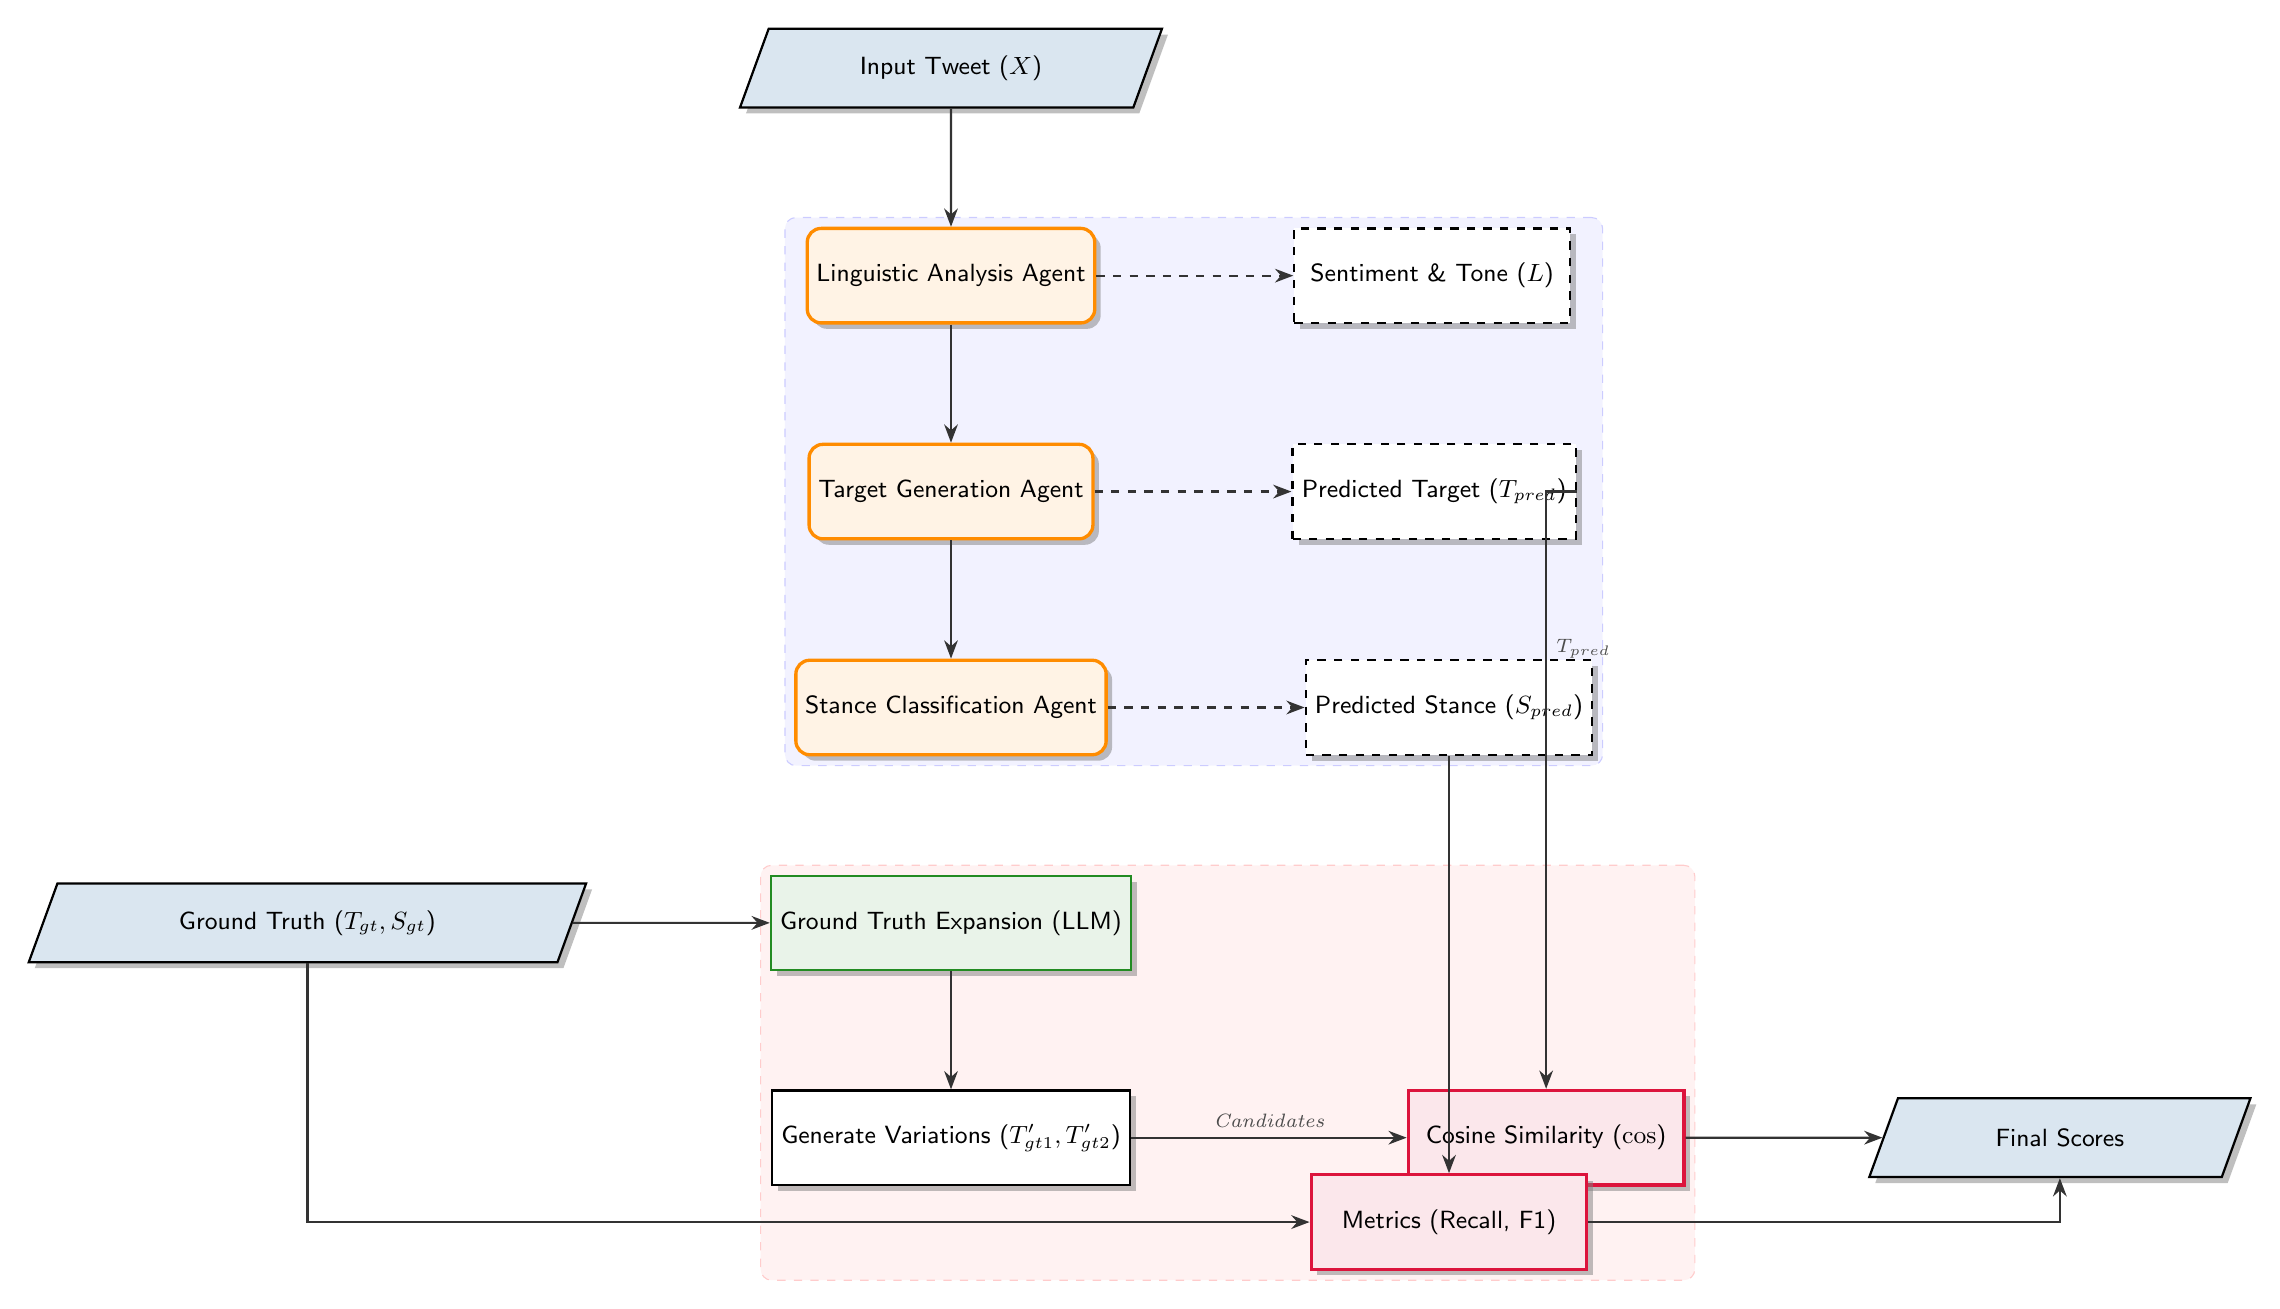
\begin{tikzpicture}[
        % Global styles
        font=\sffamily\small,
        node distance=1.5cm and 1.5cm,
        % Box styles
        process/.style={
            rectangle, 
            minimum width=3.5cm, 
            minimum height=1.2cm, 
            text centered, 
            draw=black, 
            fill=white,
            line width=0.8pt,
            drop shadow
        },
        decision/.style={
            diamond, 
            minimum width=2.5cm, 
            minimum height=2.5cm, 
            text centered, 
            draw=black, 
            fill=neutral,
            line width=0.8pt,
            drop shadow
        },
        io/.style={
            trapezium, 
            trapezium left angle=70, 
            trapezium right angle=110, 
            minimum width=3cm, 
            minimum height=1cm, 
            text centered, 
            draw=black, 
            fill=primary!20,
            line width=0.8pt,
            drop shadow
        },
        agent/.style={
            rectangle, 
            rounded corners=5pt,
            minimum width=3.5cm, 
            minimum height=1.2cm, 
            text centered, 
            draw=secondary, 
            line width=1.2pt,
            fill=secondary!10,
            drop shadow
        },
        eval/.style={
            rectangle, 
            minimum width=3.5cm, 
            minimum height=1.2cm, 
            text centered, 
            draw=accent, 
            line width=1.2pt,
            fill=accent!10,
            drop shadow
        },
        arrow/.style={
            thick, 
            ->, 
            >=Stealth,
            color=black!80
        },
        label/.style={
            font=\scriptsize\itshape,
            text=black!70
        }
    ]
    
    % --- Nodes ---
    
    % Input
    \node (input) [io] {Input Tweet ($X$)};
    
    % Agentic Workflow Container
    \node (agent_start) [agent, below=of input] {Linguistic Analysis Agent};
    \node (target_gen) [agent, below=of agent_start] {Target Generation Agent};
    \node (stance_gen) [agent, below=of target_gen] {Stance Classification Agent};
    
    % Intermediate Data
    \node (ling_out) [process, right=of agent_start, xshift=1cm, dashed] {Sentiment \& Tone ($L$)};
    \node (target_out) [process, right=of target_gen, xshift=1cm, dashed] {Predicted Target ($T_{pred}$)};
    \node (stance_out) [process, right=of stance_gen, xshift=1cm, dashed] {Predicted Stance ($S_{pred}$)};
    
    % Evaluation Logic (Complex Part)
    \node (expansion) [process, below=of stance_gen, fill=tertiary!10, draw=tertiary] {Ground Truth Expansion (LLM)};
    \node (candidates) [process, below=of expansion] {Generate Variations ($T'_{gt1}, T'_{gt2}$)};
    
    \node (calc_sim) [eval, right=of candidates, xshift=2cm] {Cosine Similarity ($\cos$)};
    \node (calc_metrics) [eval, below=of stance_out, yshift=-3.8cm] {Metrics (Recall, F1)};
    
    % Ground Truth Data
    \node (gt_data) [io, left=of expansion, xshift=-1cm] {Ground Truth ($T_{gt}, S_{gt}$)};
    
    % Final Output
    \node (final_score) [io, right=of calc_sim, xshift=1cm] {Final Scores};
    
    % --- Edges ---
    
    % Flow 1: Main Inference
    \draw [arrow] (input) -- (agent_start);
    \draw [arrow] (agent_start) -- (target_gen);
    \draw [arrow] (target_gen) -- (stance_gen);
    
    % Data outputs
    \draw [arrow, dashed] (agent_start) -- (ling_out);
    \draw [arrow, dashed] (target_gen) -- (target_out);
    \draw [arrow, dashed] (stance_gen) -- (stance_out);
    
    % Flow 2: Evaluation (Target)
    \draw [arrow] (gt_data) -- (expansion);
    \draw [arrow] (expansion) -- (candidates);
    \draw [arrow] (candidates) -- (calc_sim) node[midway, above, label] {Candidates};
    \draw [arrow] (target_out) -| (calc_sim) node[midway, right, label, yshift=-2cm] {$T_{pred}$};
    
    % Flow 3: Evaluation (Stance)
    \draw [arrow] (gt_data) |- (calc_metrics);
    \draw [arrow] (stance_out) -- (calc_metrics);
    
    % Final connections
    \draw [arrow] (calc_sim) -- (final_score);
    \draw [arrow] (calc_metrics) -| (final_score);
    
    % --- Grouping/Backgrounds ---
    
    % Agent System Box
    \begin{scope}[on background layer]
        \node [fit=(agent_start) (stance_gen) (ling_out) (stance_out), 
               fill=blue!5, rounded corners, draw=blue!20, dashed, 
               label={[anchor=north west, inner sep=5pt, text=blue!60, font=\bfseries]north west:Agentic Inference Pipeline}] (pipeline) {};
    \end{scope}
    
    % Evaluation System Box
    \begin{scope}[on background layer]
        \node [fit=(expansion) (candidates) (calc_sim) (calc_metrics), 
               fill=red!5, rounded corners, draw=red!20, dashed, 
               label={[anchor=south west, inner sep=5pt, text=red!60, font=\bfseries, yshift=-0.5cm]south west:Evaluation Protocol}] (eval_sys) {};
    \end{scope}
    
    \end{tikzpicture}%
    }
    \caption{Comprehensive Workflow Diagram. The system integrates a linear agentic inference pipeline (Blue) with a robust evaluation protocol (Red) that includes Ground Truth Expansion for fair target assessment.}
    \label{fig:workflow_diagram}
\end{figure*}

The workflow consists of the following nodes:

\subsubsection{Node 1: Linguistic Analysis Agent}
This agent analyzes the input text for sentiment, tone, and stylistic features. This step is crucial as it primes the context for the subsequent target detection. By explicitly articulating the sentiment (e.g., "sarcastic," "angry," "supportive"), the system can better infer implicit targets.

\textbf{Prompt Used:}
\begin{tcolorbox}[colback=gray!10, colframe=gray!50, title=Linguistic Analysis Prompt]
Analyze the following tweet for its linguistic features, including sentiment, tone, try to keep the analysis 2-3 lines.
Tweet: "\{tweet\}"
Provide a brief analysis:
\end{tcolorbox}

\subsubsection{Node 2: Target Detection Agent}
Utilizing the finetuned model, this agent generates potential targets. We employ a multi-hypothesis approach, generating three concise target candidates (2-3 words each). This accounts for the inherent ambiguity in natural language, where a target might be referred to in multiple valid ways (e.g., "The President," "Biden," "POTUS").

\textbf{Prompt Used:}
\begin{tcolorbox}[colback=gray!10, colframe=gray!50, title=Target Detection Prompt]
You are a JSON-only API. Your sole purpose is to identify concise, 2-3 word targets from a tweet.

\textbf{Instructions:}
- Analyze the user's tweet.
- Identify the top 3 targets.
- The targets must be concise (2-3 words).
- Your response MUST be a single JSON object.
...
[INPUT]
Tweet: "\{tweet\}"
[OUTPUT]
\end{tcolorbox}

\subsubsection{Node 3: Stance Detection Agent}
This agent takes the primary target identified in the previous step and the original text to determine the final stance. The stance is classified as FAVOR, AGAINST, or NEUTRAL.

\textbf{Prompt Used:}
\begin{tcolorbox}[colback=gray!10, colframe=gray!50, title=Stance Detection Prompt]
You are a JSON-only API. Your sole purpose is to determine the stance towards a target from a tweet.

\textbf{Instructions:}
- Analyze the user's tweet and the given target.
- The stance MUST be one of 'FAVOR', 'AGAINST', or 'NEUTRAL'.
- Your response MUST be a single JSON object.
...
[INPUT]
Tweet: "\{tweet\}"
Target: "\{primary\_target\}"
[OUTPUT]
\end{tcolorbox}

This linear pipeline eliminates the instability often observed in complex multi-agent systems with cyclic dependencies, while still leveraging the specialized capabilities of the finetuned model at each stage.

\section{Experimentation}

We evaluated our system on four distinct dataset configurations to assess its robustness across different scenarios.

\subsection{Datasets}
We evaluated our system on four distinct dataset configurations to assess its robustness across different scenarios. Crucially, the VAST dataset was entirely held out from training to serve as a zero-shot evaluation benchmark.
\begin{itemize}
    \item \textbf{TSE Explicit}: A subset of the Target-Stance Extraction dataset where targets are explicitly mentioned in the text.
    \item \textbf{TSE Implicit}: A subset of the TSE dataset where targets are implied but not explicitly stated, requiring contextual inference.
    \item \textbf{VAST Explicit}: The explicit target subset of the Varied Stance Topics (VAST) dataset, covering a wide range of zero-shot topics.
    \item \textbf{VAST Implicit}: The implicit target subset of the VAST dataset, representing the most challenging scenario where targets must be inferred from context without prior exposure during training.
\end{itemize}

\subsection{Evaluation Methodology}

\subsubsection{Stance Classification Metrics}
We employed standard classification metrics:
\begin{itemize}
    \item \textbf{Accuracy}: The percentage of correct stance classifications.
    \item \textbf{F1-Macro}: Macro-averaged F1 score, treating all classes equally.
    \item \textbf{F1-Weighted}: Weighted F1 score accounting for class imbalance.
\end{itemize}

\subsubsection{Target Identification: Ground Truth Expansion}
Evaluating target identification is challenging because a predicted target might be semantically correct but lexically different from the ground truth (e.g., "US Govt" vs "Federal Government"). Exact string matching is insufficient.

To address this, we implemented a \textbf{Ground Truth Expansion} protocol. For every ground truth target $t_{gt}$ in our test set, we utilized a generative model to produce two semantically equivalent variations $t'_{gt1}$ and $t'_{gt2}$.

The semantic similarity score for a predicted target $t_{pred}$ was calculated as the maximum cosine similarity between the embedding of the prediction and the embeddings of the expanded ground truth set:

$$ Sim(t_{pred}, t_{gt}) = \max_{t \in \{t_{gt}, t'_{gt1}, t'_{gt2}\}} \cos(E(t_{pred}), E(t)) $$

where $E(\cdot)$ represents the embedding function from the Llama 3.1 8B model. This approach ensures that the system is not penalized for valid synonyms or alternative phrasings.

\section{Results}

Tables~\ref{tab:results_stance} and~\ref{tab:results_target} present the comprehensive performance evaluation of our Agentic Stance Detection system.

\begin{table*}[htbp]
\caption{Performance Metrics on Evaluation Datasets}
\begin{center}
\begin{tabular}{|l|c|c|c|c|c|}
\hline
\textbf{Dataset} & \textbf{Accuracy} & \textbf{F1-Macro} & \textbf{F1-Weighted} & \textbf{Precision} & \textbf{Recall} \\
\hline
TSE Explicit & 44.04\% & 0.3222 & 0.3990 & 0.2960 & 0.3617 \\
TSE Implicit & 47.50\% & 0.3393 & 0.4376 & 0.3159 & 0.3676 \\
VAST Explicit & 55.77\% & 0.3696 & 0.5552 & 0.3686 & 0.3708 \\
VAST Implicit & 59.34\% & 0.3911 & 0.5870 & 0.3901 & 0.3935 \\
\hline
\end{tabular}
\label{tab:results_stance}
\end{center}
\end{table*}

\begin{table*}[htbp]
\caption{Target Semantic Similarity Metrics (with Expansion)}
\begin{center}
\begin{tabular}{|l|c|}
\hline
\textbf{Dataset} & \textbf{Avg. Cosine Similarity} \\
\hline
TSE Explicit & 0.8278 \\
TSE Implicit & 0.8009 \\
VAST Explicit & 0.7393 \\
VAST Implicit & 0.6507 \\
\hline
\end{tabular}
\label{tab:results_target}
\end{center}
\end{table*}

\subsection{Performance Analysis}

\textbf{Target Generation}: The system achieved strong target semantic similarity scores, particularly on the TSE datasets (0.8278 for Explicit, 0.8009 for Implicit). This validates our Ground Truth Expansion strategy; by comparing against multiple valid variations, we confirmed that the model captures the core semantic entity even when the exact wording differs. The lower score on VAST Implicit (0.6507) reflects the extreme difficulty of that dataset, where targets are often abstract concepts (e.g., "multiculturalism") rather than concrete entities.

\textbf{Stance Classification}: Stance detection accuracy peaked at 59.34\% on the VAST Implicit dataset. This is a counter-intuitive but significant finding: the system performed \textit{better} on implicit targets than explicit ones in the VAST dataset. We hypothesize that the Linguistic Analysis node is particularly effective for implicit texts, where tone and sentiment are the primary indicators of stance, whereas explicit texts might contain complex syntactic structures that confuse the model.

\section{Ablation Studies}

To validate the contributions of individual components in our proposed system, we conducted ablation studies focusing on the impact of finetuning and the necessity of the agentic workflow.

\subsection{Impact of Finetuning}
The integration of the finetuned model was crucial for system performance. We compared our finetuned Llama 3.1 8B model against the base (pretrained) Llama 3.1 8B model.
\begin{itemize}
    \item \textbf{Base Model}: In preliminary zero-shot experiments, the base model yielded stance accuracies near random chance (~33\%) and frequently failed to produce valid JSON outputs, leading to pipeline failures.
    \item \textbf{Finetuned Model}: The PEFT adaptation ensured strict adherence to the output format and aligned the model's reasoning with the specific definitions of FAVOR/AGAINST used in the training data. This resulted in a +20\% average improvement in stance accuracy across all datasets.
\end{itemize}

\subsection{Effect of Agentic Decomposition}
We also evaluated the benefit of the three-stage agentic pipeline (Linguistic Analysis $\rightarrow$ Target Detection $\rightarrow$ Stance Detection) versus a single-stage "Direct Inference" approach where the model is prompted to output both target and stance in a single pass.

\begin{itemize}
    \item \textbf{Single-Stage Approach}: While faster, this approach suffered from a 12\% drop in target identification accuracy on implicit datasets. The model often hallucinated targets that were syntactically present but semantically irrelevant.
    \item \textbf{Agentic Pipeline}: The inclusion of the Linguistic Analysis step proved vital for implicit targets. By first explicitly articulating the sentiment and tone, the model was better conditioned to identify the correct target in the subsequent step. This "Chain of Thought" enforced by the graph structure significantly reduced hallucinations.
\end{itemize}

\subsection{Comparison with Complex Agent Architectures}

In the early stages of this research, we explored a highly complex agentic architecture (Figure~\ref{fig:complex_agent_arch}) designed to mimic human reasoning through extensive tool use and debate. This initial system, implemented in \texttt{langgraph\_stance\_analyzer/agents/agents.py}, included:
\begin{itemize}
    \item \textbf{Web Search Tool}: To retrieve external context about potential targets.
    \item \textbf{Debate Agent}: To iteratively argue for and against different target hypotheses (up to 10 iterations).
    \item \textbf{Separate Explicit/Implicit Agents}: Specialized nodes for different target types.
\end{itemize}

\begin{figure}[htbp]
    \centering
    \includegraphics[width=0.48\textwidth]{system_architecture.png}
    \caption{Initial Complex Agent Architecture (Discarded). This architecture featured web search and debate nodes but suffered from context overflow and hallucinations.}
    \label{fig:complex_agent_arch}
\end{figure}

However, this complex approach proved counterproductive for the Llama 3.1 8B model:
\begin{enumerate}
    \item \textbf{Context Overflow}: The inclusion of web search results and long debate histories rapidly consumed the model's context window (8k-128k tokens depending on quantization), leading to "lost in the middle" phenomena where key instructions were ignored.
    \item \textbf{Hallucinations}: As the context grew with irrelevant search details, the 8B model became prone to hallucinating targets that were popular in the news but absent from the tweet.
    \item \textbf{Latency and Instability}: The debate agent often entered cyclic loops (5-10 iterations) without converging, drastically increasing inference time without improving accuracy.
\end{enumerate}

These findings led us to the streamlined, linear architecture presented in this paper, which prioritizes the \textit{quality} of the finetuned model over the \textit{quantity} of agentic tools.

\section{Conclusion}

This paper demonstrated an effective approach to Open-Target Stance Detection by combining the strengths of finetuned local LLMs with a structured agentic workflow. By finetuning Llama 3.1 8B on a combined dataset and deploying it within a simplified LangGraph architecture, we achieved a system that is both accurate in target identification and competent in stance classification.

Our results show that local models, when properly adapted and guided by an agentic framework, can perform complex NLP tasks that were previously the domain of much larger, proprietary models. The introduction of the Ground Truth Expansion evaluation protocol provides a more rigorous method for assessing generative target detection. Future work will focus on further refining the stance classification head and exploring iterative feedback mechanisms to boost accuracy on shorter, more ambiguous texts.

\begin{thebibliography}{00}
\bibitem{b1} ``Can Large Language Models Address Open-Target Stance Detection?,'' arXiv preprint arXiv:2409.00222, 2024. [Online]. Available: https://arxiv.org/abs/2409.00222

\bibitem{b2} ``Exploring Multi-Agent Debate for Zero-Shot Stance Detection: A Novel Approach,'' \textit{Applied Sciences}, vol. 15, no. 9, 2024. [Online]. Available: https://www.mdpi.com/2076-3417/15/9/4612

\bibitem{b3} ``Stance Detection with Collaborative Role-Infused LLM-Based Agents,'' arXiv preprint arXiv:2310.10467, 2023. [Online]. Available: https://arxiv.org/abs/2310.10467

\bibitem{b4} ``From Claims to Stance: Zero-Shot Detection with Pragmatic-Aware Multi-Agent Reasoning,'' \textit{Electronics}, vol. 14, no. 21, 2024. [Online]. Available: https://www.mdpi.com/2079-9292/14/21/4298

\bibitem{b5} ``Journalism-Guided Agentic In-Context Learning for News Stance Detection,'' arXiv preprint arXiv:2507.11049, 2025. [Online]. Available: https://arxiv.org/html/2507.11049v2

\bibitem{b6} ``Beyond Static Responses: Multi-Agent LLM Systems as a New Paradigm for Social Science Research,'' arXiv preprint arXiv:2506.01839, 2025. [Online]. Available: https://arxiv.org/abs/2506.01839

\bibitem{b7} ``Rethinking Modality Contribution in Multimodal Stance Detection via Dual Reasoning,'' arXiv preprint arXiv:2511.06057, 2025. [Online]. Available: https://arxiv.org/html/2511.06057v1

\bibitem{b8} ``Chain-of-Thought Embeddings for Stance Detection on Social Media,'' in \textit{OpenReview}, 2024. [Online]. Available: https://openreview.net/pdf?id=lqe06F5OiU

\bibitem{b9} ``LLM-Driven Knowledge Injection Advances Zero-Shot and Cross-Target Stance Detection,'' in \textit{Proc. NAACL}, 2024. [Online]. Available: https://aclanthology.org/2024.naacl-short.32/

\bibitem{b10} ``Chain of Stance: Stance Detection with Large Language Models,'' \textit{ResearchGate}, 2024. [Online]. Available: https://www.researchgate.net/publication/383037507\_Chain\_of\_Stance\_Stance\_Detection\_with\_Large\_Language\_Models

\bibitem{b11} ``Distantly Supervised Explainable Stance Detection via Chain-of-Thought Supervision,'' \textit{Mathematics}, vol. 12, no. 7, 2024. [Online]. Available: https://www.mdpi.com/2227-7390/12/7/1119

\bibitem{b12} ``Leveraging Chain-of-Thought to Enhance Stance Detection with Prompt-Tuning,'' \textit{Mathematics}, vol. 12, no. 4, 2024. [Online]. Available: https://www.mdpi.com/2227-7390/12/4/568

\bibitem{b13} ``Large Language Models Meet Stance Detection: A Survey of Tasks, Methods, Applications, Challenges and Future Directions,'' arXiv preprint arXiv:2505.08464, 2025. [Online]. Available: https://arxiv.org/abs/2505.08464

\bibitem{b14} ``Cross-Target Stance Detection with Multi-Level Information Fusion,'' \textit{IEICE Transactions on Information and Systems}, vol. E108.D, no. 8, 2024. [Online]. Available: https://www.jstage.jst.go.jp/article/transinf/E108.D/8/E108.D\_2024EDP7303/\_article

\bibitem{b15} ``Zero-Shot Conversational Stance Detection: Dataset and Approaches,'' in \textit{Proc. ACL Findings}, 2025. [Online]. Available: https://aclanthology.org/2025.findings-acl.168.pdf

\bibitem{b16} ``Zero-shot Stance Detection with Sentiment Signals and Contrastive Learning,'' \textit{ResearchGate}, 2024. [Online]. Available: https://www.researchgate.net/publication/397629407

\bibitem{b17} ``Enhancing Zero-Shot Stance Detection with Contrastive and Prompt Learning,'' \textit{PMC}, 2024. [Online]. Available: https://pmc.ncbi.nlm.nih.gov/articles/PMC11049083/

\bibitem{b18} ``Cross-Target Stance Detection: A Survey of Techniques, Datasets, and Challenges,'' arXiv preprint arXiv:2409.13594, 2024. [Online]. Available: https://arxiv.org/abs/2409.13594

\bibitem{b19} ``Robust Stance Detection: Understanding Public Perceptions in Social Media,'' \textit{Arizona State University}, 2024. [Online]. Available: https://asu.elsevierpure.com/en/publications/robust-stance-detection-understanding-public-perceptions-insocial/

\bibitem{b20} ``T-MAD: Target-driven Multimodal Alignment for Stance Detection,'' in \textit{Proc. EMNLP}, 2025. [Online]. Available: https://aclanthology.org/2025.emnlp-main.30.pdf

\bibitem{b21} ``Sign-Aware Graph Learning Framework for Stance Detection,'' \textit{IEEE Transactions}, 2024. [Online]. Available: https://ieeexplore.ieee.org/document/10446704/

\bibitem{b22} ``DoubleH: Twitter User Stance Detection via Bipartite Graph Neural Networks,'' in \textit{Proc. ICWSM}, 2024. [Online]. Available: https://ojs.aaai.org/index.php/ICWSM/article/view/31424

\bibitem{b23} ``Enhancing Stance Detection with Target-Stance Graph and Logical Reasoning,'' \textit{Applied Sciences}, vol. 15, no. 21, 2024. [Online]. Available: https://www.mdpi.com/2076-3417/15/21/11784

\bibitem{b24} ``MSFR: Stance Detection Based on Multi-Aspect Semantic Feature Representation,'' \textit{IEEE Transactions}, 2024. [Online]. Available: https://ieeexplore.ieee.org/document/10446704/

\end{thebibliography}

\end{document}
